% Chapitre 1 — Introduction (version française)

\chapter{Introduction}

\section{Contexte et motivation}
\label{sec:1.1}

Le Système de Noms de Domaine (DNS), spécifié par Mockapetris~\cite{RFC1034,RFC1035}, est le service d'annuaire distribué qui traduit les noms de domaine en adresses IP et sous-tend pratiquement chaque application en réseau sur Internet. Malgré cette criticité --- illustrée par la panne DNS de Facebook en octobre 2021, qui a rendu le domaine inaccessible dans le monde entier pendant près de six heures~\cite{Xu2023} --- le DNS a historiquement reçu moins d'attention systématique en termes de mesure que d'autres couches d'infrastructure. Le système de mesure DNS longitudinal le plus complet, OpenINTEL~\cite{vanRijswijk2016}, mesure quotidiennement plus de 50\,\% de l'espace de nommage DNS mondial, mais le fait depuis \textbf{un seul point de mesure aux Pays-Bas}, laissant la dimension géographique des réponses DNS entièrement non caractérisée. La figure~\ref{fig:dns_resolution} illustre le processus de résolution itératif standard.

\begin{figure}[tp]
  \centering
  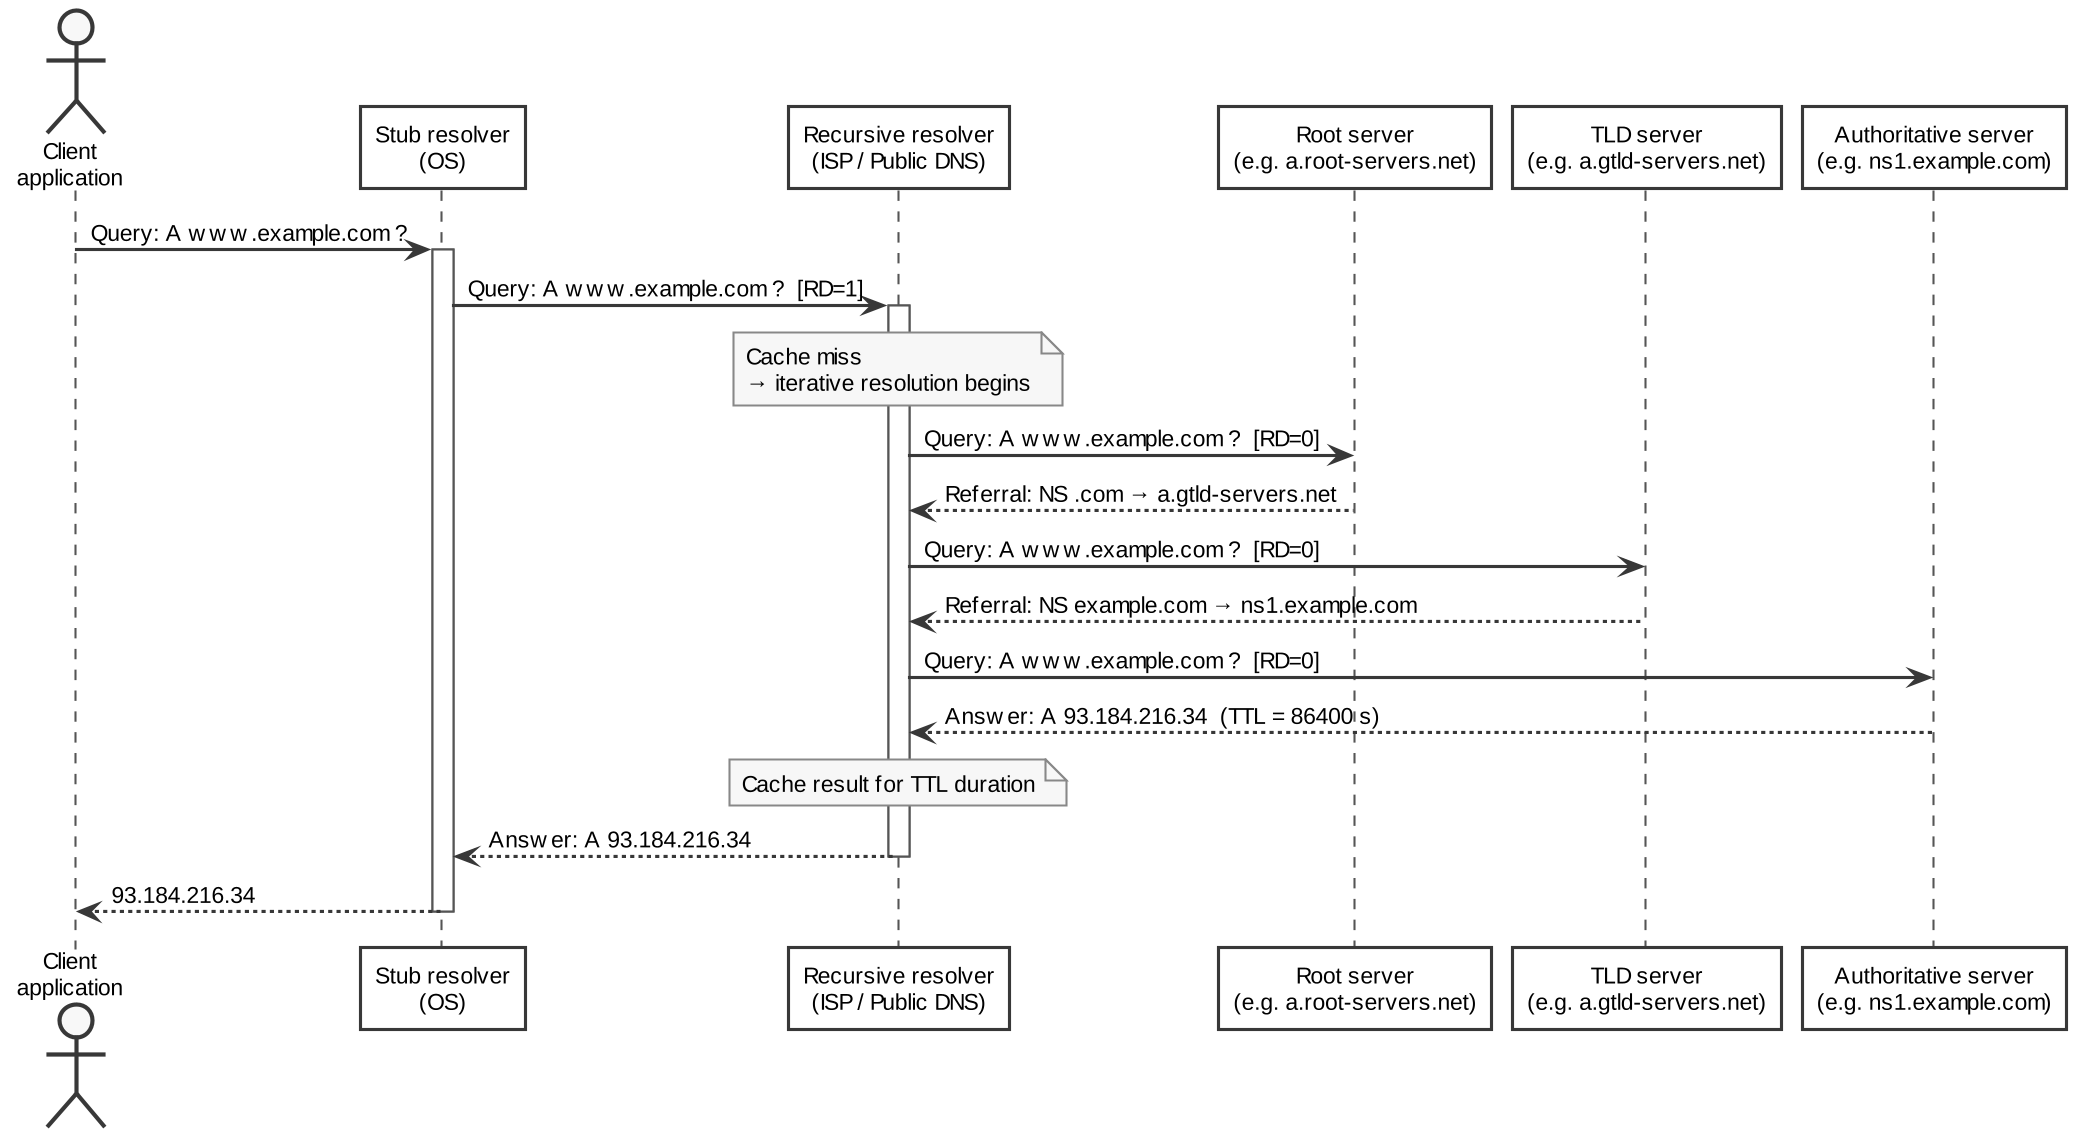
\includegraphics[width=0.92\linewidth]{figures/fig1_dns_resolution.png}
  \caption{Processus de résolution DNS itératif. Le résolveur stub transmet la requête à un résolveur récursif, qui effectue trois requêtes de référencement successives (racine $\rightarrow$ TLD $\rightarrow$ serveur faisant autorité) avant de retourner la réponse finale. Le champ TTL détermine la durée de mise en cache du résultat par le résolveur récursif.}
  \label{fig:dns_resolution}
\end{figure}

Les données DNS sont également fondamentalement \textbf{éphémères} : chaque enregistrement de ressource porte un Time To Live (TTL) après lequel il est invalidé~\cite{RFC1034,RFC1035}. Les administrateurs de zones peuvent modifier les enregistrements à tout moment, et l'infrastructure DNS ne conserve aucune trace des configurations précédentes. Cette éphémérité motive l'archivage longitudinal : les chercheurs en sécurité ont besoin de données DNS historiques pour reconstruire l'évolution des infrastructures malveillantes~\cite{vanderToorn2018} ; les chercheurs en simulation ont besoin de données historiquement précises provenant de multiples points de mesure ; les analystes d'infrastructure ont besoin de jeux de données longitudinaux pour suivre les migrations de fournisseurs et les tendances de déploiement DNSSEC~\cite{vanRijswijk2016}.

Au-delà de la dimension temporelle, les réponses DNS présentent une \textbf{dimension géographique} qu'une mesure depuis un seul point d'observation ne peut pas capturer. Trois mécanismes produisent cette variation : (1) \textbf{le routage CDN} --- les serveurs faisant autorité retournent des adresses IP différentes selon la localisation inférée du résolveur interrogeant, dirigeant les clients vers le cluster frontal le plus proche~\cite{Li2025,Hours2016} ; (2) \textbf{l'anycast IP} --- la même adresse IP globale est annoncée depuis plusieurs PoP géographiquement distribués, de sorte que les requêtes provenant de différentes régions atteignent différentes instances physiques~\cite{Bortzmeyer2013,Koch2021} ; et (3) \textbf{EDNS Client Subnet (ECS)}~\cite{RFC7871} --- le résolveur intègre un préfixe IP client tronqué dans la requête, permettant au CDN de router par localisation du client final plutôt que par localisation du résolveur~\cite{Wang2018}. La figure~\ref{fig:geographic_mechanisms} résume ces trois mécanismes.

\begin{figure}[tp]
  \centering
  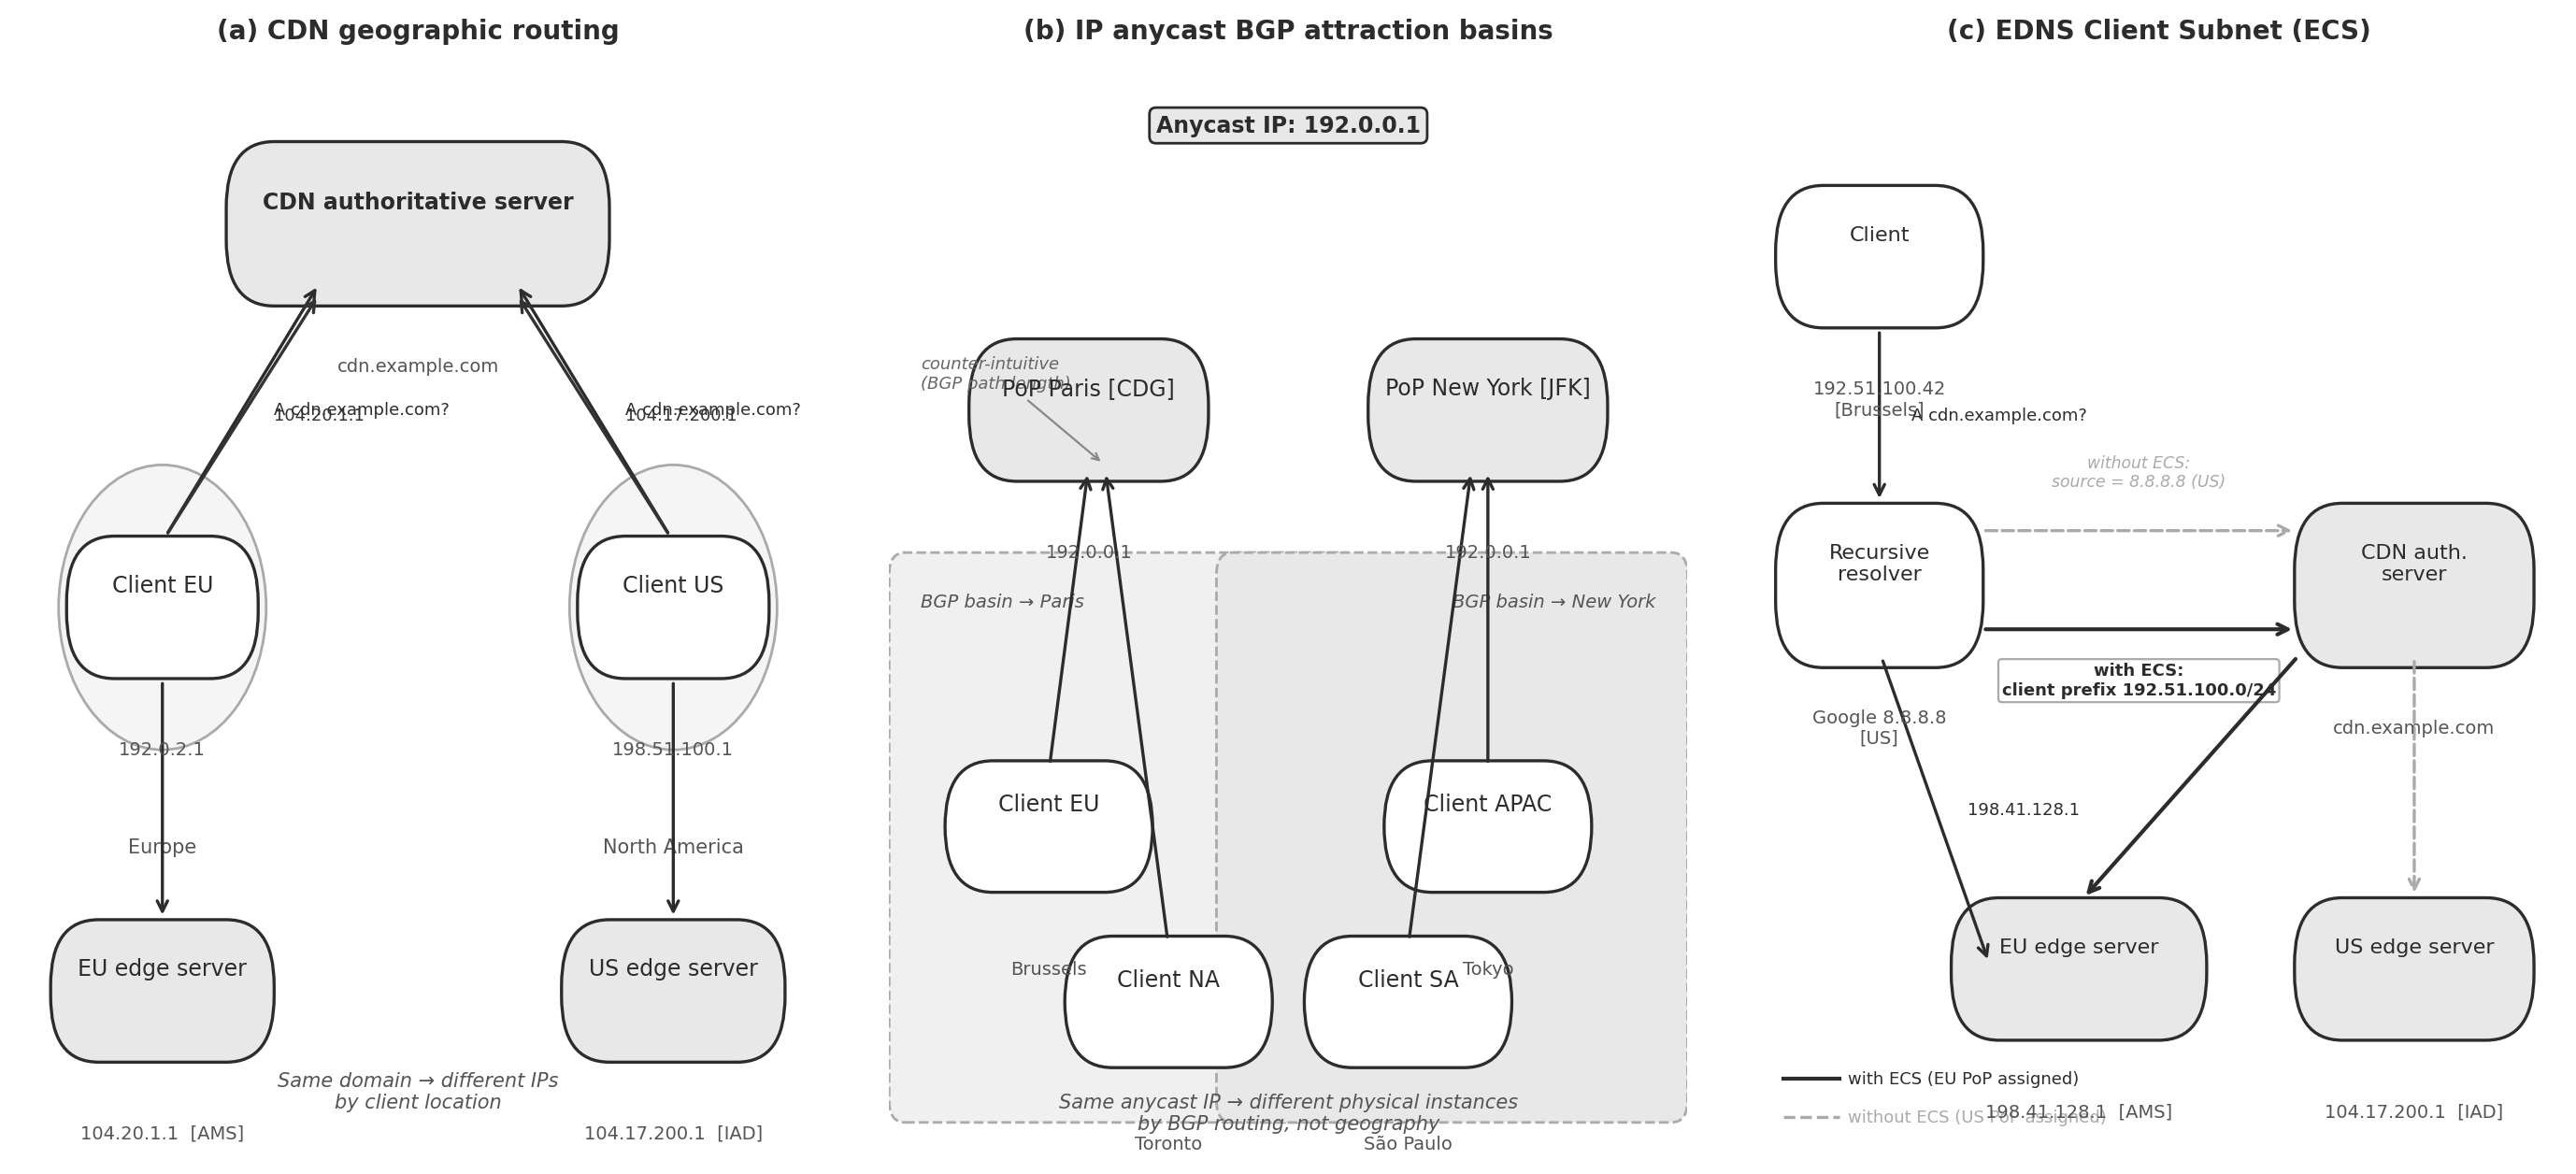
\includegraphics[width=\linewidth]{figures/fig2_geographic_mechanisms.png}
  \caption{Les trois mécanismes produisant une variation géographique dans les réponses DNS : routage CDN par IP du résolveur, bassins d'attraction BGP anycast, et EDNS Client Subnet.}
  \label{fig:geographic_mechanisms}
\end{figure}

La proportion de domaines populaires qui retournent des réponses géographiquement différenciées, l'ampleur et la stabilité temporelle de cette différenciation, et les mécanismes qui la produisent restent empiriquement non caractérisés à l'échelle de la population. C'est le manque que ce mémoire adresse.

\section{Questions de recherche et objectifs}
\label{sec:1.2}

Ce mémoire aborde la question de recherche principale suivante :

\textit{Comment concevoir et déployer un système de mesure DNS distribué qui capture la diversité géographique et temporelle des réponses DNS pour les domaines les plus populaires, de manière reproductible et utile à la communauté de recherche ?}

Quatre sous-questions opérationnelles guident l'analyse empirique :

\textbf{Q1 --- Diversité géographique} : Quelle proportion des domaines Tranco Top-10K retourne des réponses DNS différentes selon l'origine de la requête, et quels mécanismes (routage CDN, anycast, ECS) expliquent la différenciation ?

\textbf{Q2 --- Stabilité temporelle} : Quelle est la stabilité temporelle des réponses DNS aux échelles jour, semaine et mois sur la période de mesure ?

\textbf{Q3 --- Biais géographique de RIPE Atlas} : Les biais géographiques documentés de la distribution des sondes RIPE Atlas~\cite{Bajpai2017} (91\,\% des sondes en Europe/Amérique du Nord) affectent-ils significativement la capacité à observer la variation géographique DNS ?

\textbf{Q4 --- Impact du résolveur} : Quel est l'impact mesurable du choix de résolveur (ISP local ou DNS public avec ECS) sur les réponses DNS observées, et interagit-il avec la localisation de la sonde ?

Pour répondre à ces questions, le mémoire conçoit, implémente et opère un système de mesure qui : (i) mesure les 10\,000 domaines Tranco~\cite{LePochat2019} quotidiennement sur 90 jours ; (ii) collecte des mesures depuis $\approx$100 sondes RIPE Atlas distribuées globalement et sélectionnées par stratification géographique ; (iii) archive les résultats au format Avro/Parquet selon les principes FAIR ; et (iv) analyse le jeu de données pour produire des réponses quantitatives à Q1--Q4. La conception de la mesure respecte les lignes directrices éthiques de RIPE Atlas~\cite{Kisteleki2016} : tous les domaines interrogés sont publiquement accessibles, la fréquence de mesure respecte les TTL DNS, et aucun contenu politiquement sensible n'est inclus.

\section{Structure du mémoire}
\label{sec:1.3}

\textbf{Le chapitre 2} passe en revue l'état de l'art dans cinq domaines : les paradigmes de mesure DNS et l'infrastructure OpenINTEL ; la plateforme RIPE Atlas et ses biais ; le routage anycast et l'identification d'instances via NSID ; le routage DNS des CDN et ECS ; et les listes de classement de domaines, en concluant par une analyse des lacunes.

\textbf{Le chapitre 3} décrit la méthodologie complète de mesure : configuration du corpus Tranco, sélection et stratification des sondes RIPE Atlas, paramètres de mesure DNS, pipeline de collecte de données, et architecture de stockage Avro/Parquet.

\textbf{Le chapitre 4} présente les résultats empiriques de la campagne de mesure : statistiques du jeu de données et réponses à Q1--Q4 avec preuves quantitatives et visualisations.

\textbf{Le chapitre 5} discute les résultats à la lumière de la littérature, évalue les limites de l'étude, et tire des conclusions avec des directions de recherche futures.
